\chapter{Specifikacija programske potpore}
	
\section{Funkcionalni zahtjevi}
		
		\iffalse
		\textbf{\textit{dio 1. revizije}}\\
		
		\textit{Navesti \textbf{dionike} koji imaju \textbf{interes u ovom sustavu} ili  \textbf{su nositelji odgovornosti}. To su prije svega korisnici, ali i administratori sustava, naručitelji, razvojni tim.}\\
			
		\textit{Navesti \textbf{aktore} koji izravno \textbf{koriste} ili \textbf{komuniciraju sa sustavom}. Oni mogu imati inicijatorsku ulogu, tj. započinju određene procese u sustavu ili samo sudioničku ulogu, tj. obavljaju određeni posao. Za svakog aktora navesti funkcionalne zahtjeve koji se na njega odnose.}\\
		\fi
		
		\noindent \textbf{Dionici:}
		
		\begin{packed_enum}
			
			\item Voditelji udruga
			\item Šetači pasa			
			\item Zaposlenici i volonteri u udrugama
			\item Razvojni tim
			\item Administrator
			\item Javni posjetitelji
			
		\end{packed_enum}
		\vspace{5mm}
		
		\noindent \textbf{Aktori i njihovi funkcionalni zahtjevi:}
		
		
		\begin{packed_enum}
			\item  \underbar{Javni posjetitelj (inicijator) može:}
			
			\begin{packed_enum}
				
				\item pregledati listu udruga na naslovnoj stranici
				\item odabrati udrugu te pregledati: 
				\begin{packed_enum}
					
					\item  detalje profila udruge:
					\begin{packed_enum}
						\item ime udruge
						\item voditelj udruge
						\item kontakt: email adresa i broj mobitela
						\item lokacija
						\item OIB udruge
						\item IBAN udruge - u slučaju da netko želi napraviti donaciju
					\end{packed_enum}
					\item  listu pasa iz te udruge koji su raspoloživi za šetnju
				\end{packed_enum}
			
				\item odabrati profil psa iz liste pasa te pregledati detalje profila psa: 
				\begin{packed_enum}
					\item ime psa
					\item vrsta psa (ako je poznata)
					\item slika psa
					\item opis psa (osobnost, izgled)
					\item dob psa
					\item raspored odnosno raspoloživost psa za određeni vremenski period (datum i vrijeme) 
					\item vrsta šetnje za koju je pas predodređen (skupna ili individualna)
				\end{packed_enum} 
				\item otvoriti statistiku svih pasa raspoloživih za šetnju i vidjeti koji pas se najmanje šteao, odnosno kojem psu je šetnja najpotrebnija
				\item  otvoriti rang-listu svih registriranih šetača poredanu s obzirom na broj šetnji, broj pasa te duljinu šetnje koju su odradili u proteklih mjesec dana
				\item registrirati se u sustav kao građanin - za stvaranje korisničkog računa potrebni su mu:
				\begin{packed_enum}
					\item ime i prezime
					\item e-mail adresa
					\item korisničko ime
					\item lozinka 
				\end{packed_enum}
				\item registrirati u sustav svoju udrugu - za stvaranje korisničkog računa potrebni su mu:
				\begin{packed_enum}
					\item ime i prezime
					\item e-mail adresa
					\item korisničko ime
					\item lozinka 
					\item naziv udruge
					\item OIB udruge
				\end{packed_enum}
			
				
			\end{packed_enum}
			\vspace{5mm}
			
			\item  \underbar{Registrirani korisnik (inicijator)} preuzima sve funkcionalnosti javnog posjetitelja (osim registracije) te može dodatno:
			\begin{packed_enum}
				\item prijaviti se u sustav (s e-mailom i lozinkom)
				\item uz uvjet da je prijavljen u sustav:
				\item[]
				\begin{packed_enum}
					\item pregledati vlastiti profil
					\item uređivati vlastiti profil
					\item obrisati vlastiti profil
				\end{packed_enum}	
			\end{packed_enum}
			\vspace{5mm}
		
			\item  \underbar{Registrirani građanin (inicijator)} preuzima sve funkcionalnosti registriranog korisnika te (uz uvjet da je prijavljen) može još dodatno:
			\begin{packed_enum}
				\item odabrati psa te na njegovom profilu prijaviti se za šetnju
				\item pregledati vlastiti raspored šetnji te skinuti (eng. download) raspored za odabrani dan, tjedan ili mjesec, u PDF obliku
				\item pregledati vlastitu statistiku šetanja
				\item označiti vlastite statistike šetanja kao \underbar{javne} kako bi podaci građana dospjeli na rang listu na javnoj stranici
			\end{packed_enum}
			\vspace{5mm}
		
			\item  \underbar{Registrirana udruga (inicijator)} preuzima sve funkcionalnosti registriranog korisnika te (uz uvjet da je prijavljena) može dodatno:
			\begin{packed_enum}
				\item dodavati i brisati pse iz liste raspoloživih pasa te udruge
				\item uređivati profile pasa koji su iz te udruge 
			\end{packed_enum}
			\vspace{5mm}
		
			\item \underbar{Administrator (inicijator) može:} 
			\begin{packed_enum}
				\item vidjeti popis svih registriranih korisnika i njihovih osobnih podataka
				\item brisati korisnike
			\end{packed_enum}
		
			\item  \underbar{Baza podataka (sudionik)}:
			\begin{packed_enum}
				\item pohranjuje sve podatke o korisnicima i udrugama 
				\item pohranjuje sve podatke o šetnjama (obavljenim i rezerviranim) te o psima iz udruga 
			\end{packed_enum}
		
		\end{packed_enum}
		
		\eject 
		
		
			
		\subsection{Obrasci uporabe}
		\vspace{5mm}
			
		
			
			\noindent \underbar{\textbf{\hypertarget{UC1}{UC1} - Pregled profila udruga i pasa iz te udruge}}
			\begin{packed_item}
				
				\item \textbf{Glavni sudionik:} Javni posjetitelj
				\item  \textbf{Cilj:} Otvoriti profil pojedine udruge ili psa iz te udruge
				\item  \textbf{Sudionici:} Baza podataka
				\item  \textbf{Preduvjet:} Pristup aplikaciji
				\item  \textbf{Opis osnovnog tijeka:}
				
				\item[] \begin{packed_enum}
					
					\item Korisnik sa naslovne strane odabire udrugu koju želi proučiti
					\item Iz liste pasa te udruge korisnik odabire psa koji ga zanima
					\item Korisnik može proučavati podatke, raspored i statistiku šetanja željenog psa
				\end{packed_enum}
			\end{packed_item}
		
		
			\noindent \underbar{\textbf{\hypertarget{UC2}{UC2} - Pregled liste profila svih pasa}}
			\begin{packed_item}
				
				\item \textbf{Glavni sudionik:} Javni posjetitelj
				\item  \textbf{Cilj:} Otvoriti profil psa iz bilo koje udruge
				\item  \textbf{Sudionici:} Baza podataka
				\item  \textbf{Preduvjet:} Pristup aplikaciji
				\item  \textbf{Opis osnovnog tijeka:}
				
				\item[] \begin{packed_enum}
					
					\item Korisnik iz izborne trake odabire "Lista svih pasa"
					\item Iz liste pasa korisnik odabire psa koji ga zanima
					\item Korisnik može proučavati podatke, raspored i statistiku šetanja željenog psa
				\end{packed_enum}
			\end{packed_item}
		
		
		
			\noindent \underbar{\textbf{UC3 - Pregled statistike svih pasa}}
			\begin{packed_item}
				
				\item \textbf{Glavni sudionik:} Javni posjetitelj
				\item  \textbf{Cilj:} Otvoriti statistiku šetanja svih pasa
				\item  \textbf{Sudionici:} Baza podataka
				\item  \textbf{Preduvjet:} Pristup aplikaciji
				\item  \textbf{Opis osnovnog tijeka:}
				
				\item[] \begin{packed_enum}
					
					\item Korisnik iz izborne trake odabire "Lista svih pasa"
					\item Korisnik odabire opciju "Statistika svih pasa"
					\item Korisnik može proučiti statistiku šetanja svih pasa 
				\end{packed_enum}
			\end{packed_item}
		
		\newpage
			
				
			\noindent \underbar{\textbf{UC4 - Pregled rang-liste svih šetača}}
			\begin{packed_item}
				
				\item \textbf{Glavni sudionik:} Javni posjetitelj
				\item  \textbf{Cilj:} Dobiti uvid u rang-listu svih šetača
				\item  \textbf{Sudionici:} Baza podataka
				\item  \textbf{Preduvjet:} Pristup aplikaciji
				\item  \textbf{Opis osnovnog tijeka:}
				
				\item[] \begin{packed_enum}
					
					\item Korisnik iz izborne trake odabire "Rang-lista šetača"
					\item Aplikacija prikazuje poredak šetača s obzirom na broj šetnji, broj pasa te duljinu šetnji koje su odradili u prethodnih mjesec dana
					\item Korisnik može proučiti rang-listu svih šetača
				\end{packed_enum}
				\item  \textbf{Opis mogućih odstupanja:}
				\item[] \begin{packed_item}
					\item [2.a] U slučaju da nijedan šetač nije označio statistiku svoje šetnje kao javnu, rang lista će biti prazna
				\end{packed_item}
			\end{packed_item}
	
	
	

	
			\noindent \underbar{\textbf{UC5 - Registracija korisnika (građanina ili udruge) u sustav}}
			\begin{packed_item}
				
				\item \textbf{Glavni sudionik:} Javni posjetitelj
				\item  \textbf{Cilj:} Stvoriti korisnički račun za pristup sustavu
				\item  \textbf{Sudionici:} Baza podataka
				\item  \textbf{Preduvjet:} Pristup aplikaciji
				\item  \textbf{Opis osnovnog tijeka:}
				
				\item[] \begin{packed_enum}
					
					\item Javni posjetitelj odabire opciju (gumb) za registraciju 
					\item Javni posjetitelj bira "Registriraj se kao građanin" ili "Registriraj se kao udruga"
					\item Javni posjetitelj unosi potrebne korisničke podatke (ime, prezime, korisničko ime, email adresa i lozinka za građanina te dodatno ime udruge i OIB udruge za udrugu)
					\item Javni posjetitelj odabire opciju "Stvori korisnički račun"
					\item Korisnik prima obavijest o uspješnoj registraciji
				\end{packed_enum}
				
				\item  \textbf{Opis mogućih odstupanja:}
				
				\item[] \begin{packed_item}
					
					\item [2.a] Unos podataka u neispravnom formatu 
					\item[] \begin{packed_enum}
						
						\item Sustav obavještava korisnika o neispravnim podatcima i vraća ga na stranicu za registraciju
						\item Korisnik mijenja potrebne podatke te završava unos ili odustaje od registracije

					\end{packed_enum}
					\item [2.b] Odabrana email adresa i/ili korisničko ime su već zauzeti
					\item[] \begin{packed_enum}
					
						\item Sustav obavještava korisnika o zauzetom korisničkom imenu/email adresi i vraća ga na stranicu za registraciju
						\item Korisnik mijenja potrebne podatke te završava unos ili odustaje od registracije
					
				\end{packed_enum}
				\end{packed_item}
			\end{packed_item}
		
		
		
			\noindent \underbar{\textbf{UC6 - Prijava korisnika (građanina ili udruge) u sustav}}
			\begin{packed_item}
				
				\item \textbf{Glavni sudionik:} Registrirani korisnik (građanin/udruga)
				\item  \textbf{Cilj:} Dobiti pristup odgovarajućem korisničkom sučelju
				\item  \textbf{Sudionici:} Baza podataka
				\item  \textbf{Preduvjet:} Registracija građanina ili udruge u sustav
				\item  \textbf{Opis osnovnog tijeka:}
				
				\item[] \begin{packed_enum}
					
					\item Unos korisničkog imena i lozinke
					\item Potvrda o ispravnosti unesenih podataka
					\item Pristup odgovarajućim korisničkim funkcijama (ovisi prijavljuje li se građanin ili udruga)
				\end{packed_enum}
				
				\item  \textbf{Opis mogućih odstupanja:}
				
				\item[] \begin{packed_item}
					
					\item [2.a] Neispravno korisničko ime/lozinka
					\item[] \begin{packed_enum}
						
						\item Sustav obavještava korisnika o neuspjelom upisu i vraća ga na stranicu za prijavu
						
					\end{packed_enum}
				\end{packed_item}
			\end{packed_item}
		
		
				\noindent \underbar{\textbf{UC7 - Pregled osobnih podataka korisnika (udruge ili građanina)}}
			\begin{packed_item}
				
				\item \textbf{Glavni sudionik:} Registrirani korisnik (udruga/građanin)
				\item  \textbf{Cilj:} Pregledati osobne podatke/podatke udruge
				\item  \textbf{Sudionici:} Baza podataka
				\item  \textbf{Preduvjet:} Registrirani korisnik (udruga ili građanin) je prijavljen u sustav
				\item  \textbf{Opis osnovnog tijeka:}
				
				\item[] \begin{packed_enum}	
					\item Korisnik iz izborne trake odabire "Osobni podatci"
					\item Otvara se stranica sa korisnikovim osobnim podatcima
				\end{packed_enum}
			\end{packed_item}
		
		
		
				\noindent \underbar{\textbf{UC8 - Promjena osobnih podataka korisnika}}
			\begin{packed_item}
				
				\item \textbf{Glavni sudionik:} Registrirani korisnik (udruga/građanin)
				\item  \textbf{Cilj:} Promijeniti osobne podatke/podatke udruge
				\item  \textbf{Sudionici:} Baza podataka
				\item  \textbf{Preduvjet:} Registrirani korisnik (udruga ili građanin) je prijavljen u sustav
				\item  \textbf{Opis osnovnog tijeka:}
				
				\item[] \begin{packed_enum}
					\item Korisnik iz izborne trake odabire "Osobni podatci"
					\item Otvara se stranica sa korisnikovim osobnim podatcima
					\item Korisnik bira "Uredi profil"
					\item Korisnik mijenja podatke
					\item Korisnik bira opciju "Pohrani promjene"
					\item Baza se ažurira
				\end{packed_enum}
				
				\item  \textbf{Opis mogućih odstupanja:}
				
				\item[] \begin{packed_item}
					
					\item [4.a]  Korisnik promijeni svoje osobne podatke, ali ne odabere opciju ”Pohrani
					promjene”
					\item[] \begin{packed_enum}
						
						\item Sustav upozorava korisnika da nije spremio podatke prije izlaska iz prozora
						\item Korisnik se vraća i pohranjuje promjene ili izlazi iz prozora ostavljajući podatke bez promjene
					\end{packed_enum}
				
					\item [4.b]  Korisnik promijeni svoje osobne podatke, ali u neispravan format
					\item[] \begin{packed_enum}
						
						\item Sustav upozorava korisnika da je podatak u neispravnom formatu i ne dopušta pohranu takvih podataka
						\item Korisnik mijenja podatak i pohranjuje promjene ili izlazi iz prozora ostavljajući podatke bez promjene
					\end{packed_enum}
					
						\item [6.b]  Korisnik promijeni svoje osobne podatke, ali je nova email adresa i/ili korisničko ime već zauzeto
					\item[] \begin{packed_enum}
						
						\item Sustav upozorava korisnika da je email adresa i/ili korisničko već zauzeto i da promjene ne mogu biti pohranjene
						\item Korisnik mijenja email adresu i/ili korisničko ime i pohranjuje promjene ili izlazi iz prozora ostavljajući podatke bez promjene
					\end{packed_enum}
				\end{packed_item}
			\end{packed_item}
		
		
				\noindent \underbar{\textbf{UC9 - Brisanje korisničkog računa (udruge ili građanina)}}
			\begin{packed_item}
				
				\item \textbf{Glavni sudionik:} Registrirani korisnik (udruga/građanin)
				\item  \textbf{Cilj:} Izbrisati vlastiti korisnički račun
				\item  \textbf{Sudionici:} Baza podataka
				\item  \textbf{Preduvjet:} Registrirani korisnik (udruga ili građanin) je prijavljen u sustav
				\item  \textbf{Opis osnovnog tijeka:}
				
				\item[] \begin{packed_enum}	
					\item Korisnik iz izborne trake odabire "Osobni podatci"
					\item Otvara se stranica sa korisnikovim osobnim podatcima
					\item Korisnik bira "Uredi profil"
					\item Korisnik bira "Izbriši korisniči račun"
					\item Sustav upozorava korisnika da je brisanje korisničkog računa trajno te provjerava je li siguran
					\item Korisnik potvrđuje brisanje
					\item Korisnički račun se briše iz baze podataka
					\item Otvara se naslovna stranica
				\end{packed_enum}
				\item  \textbf{Opis mogućih odstupanja:}
				
				\item[] \begin{packed_item}
					
					\item [5.a]  Korisnik poništi brisanje računa
					\item[] \begin{packed_enum}
						\item Račun se ne briše te se baza ne ažurira
						\item Korisnik je ostavljen na stranici "Uredi profil"
					\end{packed_enum}
				\end{packed_item}
			\end{packed_item}
		
			
				\noindent \underbar{\textbf{UC10 - Dodavanje novog profila psa u listu prijavljene udruge}}
			\begin{packed_item}
				
				\item \textbf{Glavni sudionik:} Registrirana udruga
				\item  \textbf{Cilj:} Dodati profil nekog psa iz te (prijavljene) udruge
				\item  \textbf{Sudionici:} Baza podataka
				\item  \textbf{Preduvjet:} Registrirana udruga je prijavljena u sustav
				\item  \textbf{Opis osnovnog tijeka:}
				
				\item[] \begin{packed_enum}
					\item Korisnik iz izborne trake odabire "Moji psi"
					\item Otvara se lista svih pasa iz te udruge
					\item Korisnik bira opciju "Dodaj novog psa"
					\item Otvara se stranica za upis podataka o novom psu 
					\item Korisnik upiše podatke, opcionalno dodaje i sliku
					\item Korisnik bira opciju "Dodaj psa"
					\item Baza se ažurira
				\end{packed_enum}
				
				\item  \textbf{Opis mogućih odstupanja:}
				
				\item[] \begin{packed_item}
					
					\item [4.a]  Korisnik upiše podatke o psu, ali ne odabere opciju "Dodaj psa"
					\item[] \begin{packed_enum}
						
						\item Sustav upozorava korisnika da nije spremio nove podatke prije izlaska iz prozora
						\item Korisnik se vraća i pohranjuje podatke ili izlazi iz prozora bez dodavanja novog psa
					\end{packed_enum}
					
					\item [4.b]  Korisnik upiše podatke o psu, ali novi podatci su u neispravanom formatu
					\item[] \begin{packed_enum}
						
						\item Sustav upozorava korisnika da je podatak (ili više njih) u neispravnom formatu i ne dopušta pohranu takvih podataka
						\item Korisnik mijenja podatak/e i pohranjuje ih ili izlazi iz prozora bez dodavanja novog psa
					\end{packed_enum}
				\end{packed_item}
			\end{packed_item}
		
		
				\noindent \underbar{\textbf{UC11 - Uređivanje profila psa neke udruge}}
			\begin{packed_item}
				
				\item \textbf{Glavni sudionik:} Registrirana udruga
				\item  \textbf{Cilj:} Urediti profil nekog psa iz te (prijavljene) udruge
				\item  \textbf{Sudionici:} Baza podataka
				\item  \textbf{Preduvjet:} Registrirana udruga je prijavljena u sustav
				\item  \textbf{Opis osnovnog tijeka:}
				
				\item[] \begin{packed_enum}
					\item Korisnik iz izborne trake odabire "Moji psi"
					\item Otvara se lista svih pasa iz te udruge
					\item Korisnik bira psa čiji profil želi urediti
					\item Korisnik mijenja podatke 
					\item Korisnik bira opciju "Pohrani promjene"
					\item Baza se ažurira
				\end{packed_enum}
				
				\item  \textbf{Opis mogućih odstupanja:}
				
				\item[] \begin{packed_item}
					
					\item [4.a]  Korisnik promijeni podatke o psu, ali ne odabere opciju ”Pohrani
					promjene”
					\item[] \begin{packed_enum}
						
						\item Sustav upozorava korisnika da nije spremio podatke prije izlaska iz prozora
						\item Korisnik se vraća i pohranjuje promjene ili izlazi iz prozora ostavljajući podatke bez promjene
					\end{packed_enum}
					
					\item [4.b]  Korisnik promijeni podatke o psu, ali novi podatci su u neispravanom formatu
					\item[] \begin{packed_enum}
						
						\item Sustav upozorava korisnika da je podatak (ili više njih) u neispravnom formatu i ne dopušta pohranu takvih podataka
						\item Korisnik mijenja podatak/e i pohranjuje promjene ili izlazi iz prozora ostavljajući podatke bez promjene
					\end{packed_enum}
				\end{packed_item}
			\end{packed_item}
		
		
			\noindent \underbar{\textbf{UC12 - Brisanje profila psa iz liste neke udruge}}
		\begin{packed_item}
			
			\item \textbf{Glavni sudionik:} Registrirana udruga
			\item  \textbf{Cilj:} Obrisati profil nekog psa iz liste pasa te (prijavljene) udruge
			\item  \textbf{Sudionici:} Baza podataka
			\item  \textbf{Preduvjet:} Registrirana udruga je prijavljena u sustav
			\item  \textbf{Opis osnovnog tijeka:}
			
			\item[] \begin{packed_enum}
				\item Korisnik iz izborne trake odabire "Moji psi"
				\item Otvara se lista svih pasa iz te udruge
				\item Korisnik bira psa čiji profil želi obrisati
				\item Korisnik bira opciju "Obriši profil psa" 
				\item Sustav šalje upit korisniku je li siguran
				\item Korisnik potvrđuje brisanje
				\item Profil tog psa se briše iz baze podataka
				\item Otvara se stranica "Moji psi"
			\end{packed_enum}
			\item  \textbf{Opis mogućih odstupanja:}
			
			\item[] \begin{packed_item}
				
				\item [5.a]  Korisnik poništi brisanje profila psa
				\item[] \begin{packed_enum}
					\item Profil psa se ne briše te se baza ne ažurira
					\item Korisnik je ostavljen na stranici "Uredi profil psa"
				\end{packed_enum}
			\end{packed_item}
		\end{packed_item}
	
	
	
		\noindent \underbar{\textbf{UC13 - Rezervacija termina šetnje}}
	\begin{packed_item}
		
		\item \textbf{Glavni sudionik:} Registrirani građanin (šetač)
		\item  \textbf{Cilj:} Šetač rezervira psa i termin u kojem će obaviti šetnju tog psa
		\item  \textbf{Sudionici:} Baza podataka
		\item  \textbf{Preduvjet:} Registrirani građanin (šetač) je prijavljen u sustav
		\item  \textbf{Opis osnovnog tijeka:}
		
		\item[] \begin{packed_enum}
			\item Šetač dolazi na stranicu za odabir profila psa preko:
				\item[] \begin{packed_enum}
					\item profila neke udruge (\hyperlink{UC1}{UC1})
					\item liste svih pasa (\hyperlink{UC2}{UC2})
				\end{packed_enum}
			\item Šetač odabire psa kojeg želi šetati
			\item Šetač dobiva uvid u slobodne termine odabranog psa te bira neki
			\item Sustav šalje potvrdu rezervacije termina šetaču
			\item Nakon uspješne rezervacije, termin za odabranog psa vidljiv je na kalendaru šetaču
		\end{packed_enum}
		\item  \textbf{Opis mogućih odstupanja:}
		
		\item[] \begin{packed_item}
			
			\item [4.a]  Odabrani pas nema slobodnih termina za šetnje
			\item[] \begin{packed_enum}
				\item Šetač izlazi iz profila psa i može tražiti novog psa za šetnju
			\end{packed_enum}
		\end{packed_item}
	\end{packed_item}


	\noindent \underbar{\textbf{UC14 - Pregled vlastitih statistika šetnji}}
	\begin{packed_item}
		
		\item \textbf{Glavni sudionik:} Registrirani građanin (šetač)
		\item  \textbf{Cilj:} Pregledati svoju statistiku šetnji u određenom razdoblju
		\item  \textbf{Sudionici:} Baza podataka
		\item  \textbf{Preduvjet:} Registrirani građanin (šetač) je prijavljen u sustav
		\item  \textbf{Opis osnovnog tijeka:}
		
		\item[] \begin{packed_enum}
			\item Šetač bira opciju "Moj profil" na izbornoj traci odnosno odlazi na stranicu svog profila
			\item Šetač odabire opciju "Moja statistika" na stranici profila
			\item Šetač bira razdoblje u kojem želi pregledati statistiku
			\item Statistika je prikazana te ju šetač može proučiti 
		\end{packed_enum}
	\end{packed_item}

\newpage
	
	\noindent \underbar{\textbf{UC15 - Označavanje statistike šetnji kao javne}}
	\begin{packed_item}
		
		\item \textbf{Glavni sudionik:} Registrirani građanin (šetač)
		\item  \textbf{Cilj:} Učiniti svoju statistiku šetnji javno dostupnom kako bi se mogla prikazati na rang-listi šetača
		\item  \textbf{Sudionici:} Baza podataka
		\item  \textbf{Preduvjet:} Registrirani građanin (šetač) je prijavljen u sustav
		\item  \textbf{Opis osnovnog tijeka:}
		
		\item[] \begin{packed_enum}
			\item Šetač bira opciju "Moj profil" na izbornoj traci odnosno odlazi na stranicu svog profila
			\item Šetač odabire opciju "Moja statistika" na stranici profila te se prikazuje stranica njegove statistike
			\item Šetač odabire opciju "Označi svoju statistiku javnom" 
			\item Njegova statistika je prikazana na javnoj rang-listi šetača
		\end{packed_enum}
	\end{packed_item}




	\noindent \underbar{\textbf{UC16 - Pregled i skidanje (eng.download) kalendara registriranog građanina}}
	\begin{packed_item}
		
		\item \textbf{Glavni sudionik:} Registrirani građanin (šetač)
		\item  \textbf{Cilj:} Pregledati svoj kalendar odnosno raspored rezerviranih šetnji i skinuti raspored za dan, mjesec ili godinu u PDF-u
		\item  \textbf{Sudionici:} Baza podataka
		\item  \textbf{Preduvjet:} Registrirani građanin (šetač) je prijavljen u sustav
		\item  \textbf{Opis osnovnog tijeka:}
		
		\item[] \begin{packed_enum}
			\item Šetač bira opciju "Moj profil" na izbornoj traci odnosno odlazi na stranicu svog profila
			\item Šetač odabire opciju "Moj kalendar" na stranici profila
			\item Šetač može birati želi li vidjeti raspored za dan, mjesec ili godinu
			\item Šetač može skinuti odabrani raspored u PDF-u
		\end{packed_enum}
	\end{packed_item}


	\noindent \underbar{\textbf{UC17 - Pregled korisnika}}
	\begin{packed_item}
		
		\item \textbf{Glavni sudionik:} Administrator
		\item  \textbf{Cilj:} Pregledati registrirane korisnike
		\item  \textbf{Sudionici:} Baza podataka
		\item  \textbf{Preduvjet:} Korisnik je registriran i dodijeljena su mu prava administratora
		\item  \textbf{Opis osnovnog tijeka:}
		
		\item[] \begin{packed_enum}
			\item Administrator bira opciju pregledavanja korisnika
			\item Prikaže se lista svih ispravno registriranih korisnika s osobnim podacima
		\end{packed_enum}
	\end{packed_item}


	\noindent \underbar{\textbf{UC18 - Brisanje korisnika korisnika}}
	\begin{packed_item}
		
		\item \textbf{Glavni sudionik:} Administrator
		\item  \textbf{Cilj:} Obrisati korisnika
		\item  \textbf{Sudionici:} Baza podataka
		\item  \textbf{Preduvjet:} Korisnik je registriran i dodijeljena su mu prava administratora
		\item  \textbf{Opis osnovnog tijeka:}
		
		\item[] \begin{packed_enum}
			\item Administrator bira opciju uklanjanja korisnika
			\item Administrator pronalazi željenog korisnika
			\item Administrator uklanja željenog korisnika i njegove podatke iz baze podataka
		\end{packed_enum}
	\end{packed_item}
		

		\subsubsection{Dijagrami obrazaca uporabe}
				
				\begin{figure}[H]
					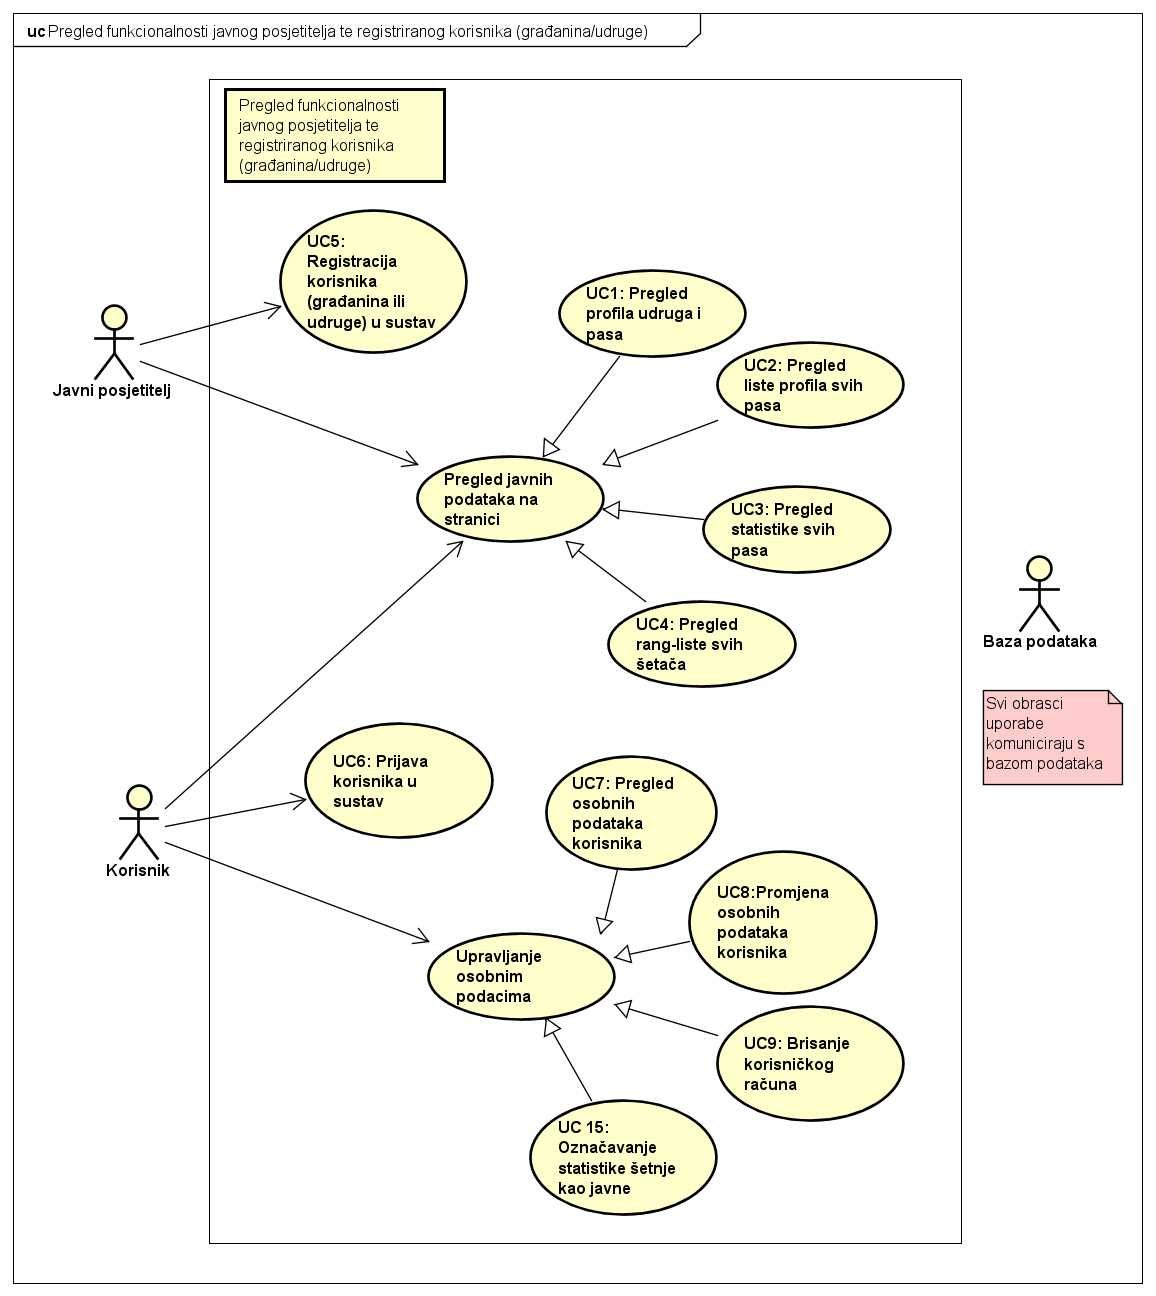
\includegraphics[scale=0.55]{dijagrami/usecase1.PNG} %veličina u odnosu na širinu linije
					\caption{Dijagram obrasca uporabe: Prikaz funkcionalnosti javnog posjetitelja te  registriranog korisnika}
					\label{fig:usecase1} %label mora biti drugaciji za svaku sliku
				\end{figure}
			
				\begin{figure}[H]
					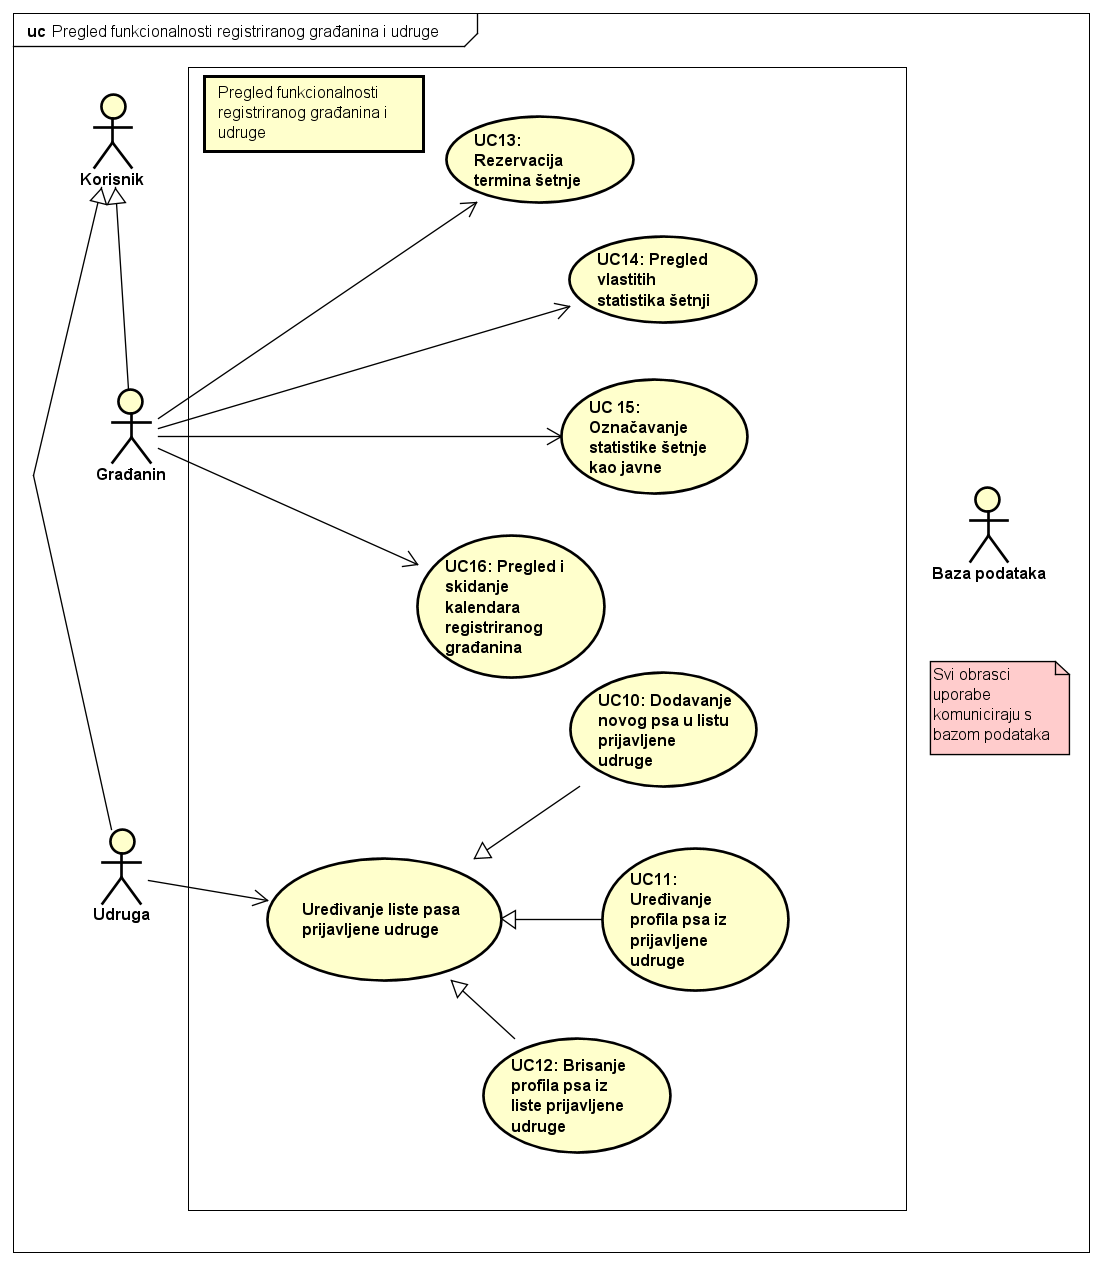
\includegraphics[scale=0.55]{dijagrami/usecase2.PNG} %veličina u odnosu na širinu linije
					\caption{Dijagram obrasca uporabe: Prikaz funkcionalnosti registriranog građanina i udruge}
					\label{fig:usecase2} %label mora biti drugaciji za svaku sliku
				\end{figure}
		\eject	
			
		\subsection{Sekvencijski dijagrami}
			\iffalse
			\textbf{\textit{dio 1. revizije}}\\
			
			\textit{Nacrtati sekvencijske dijagrame koji modeliraju najvažnije dijelove sustava (max. 4 dijagrama). Ukoliko postoji nedoumica oko odabira, razjasniti s asistentom. Uz svaki dijagram napisati detaljni opis dijagrama.}
			\eject
			\fi
			\subsubsection{Obrazac uporabe UC8: Promjena osobnih podataka korisnika}
			Korisnik šalje zahtjev za prikaz osobnih podataka. Poslužitelj dohvaća osobne podatke te ih prikazuje. Korisnik zatraži uređivanje osobnih podataka te mu aplikacija ponudi obrazac za promjenu podataka. Korisnik ispunjava podatke te bira "Spremi podatke". Ako su podaci u nesipravnom formatu, aplikacija ga upozorava na to. Ako korisnik uredi podatke u ispravan format, podaci se šalju bazi. U slučaju da je nova email adresa već zauzeta, baza šalje upozorenje aplikaciji, a aplikacija korisniku. Ako su podaci ispravni, aplikacija šalje korisniku poruku da su podaci uspješno izmijenjeni. U slučaju da korisnik izađe iz obrasca za uređivanje osobnih podataka, aplikacija korisniku šalje upozorenje da podaci nisu spremljeni.
			\begin{figure}[H]
				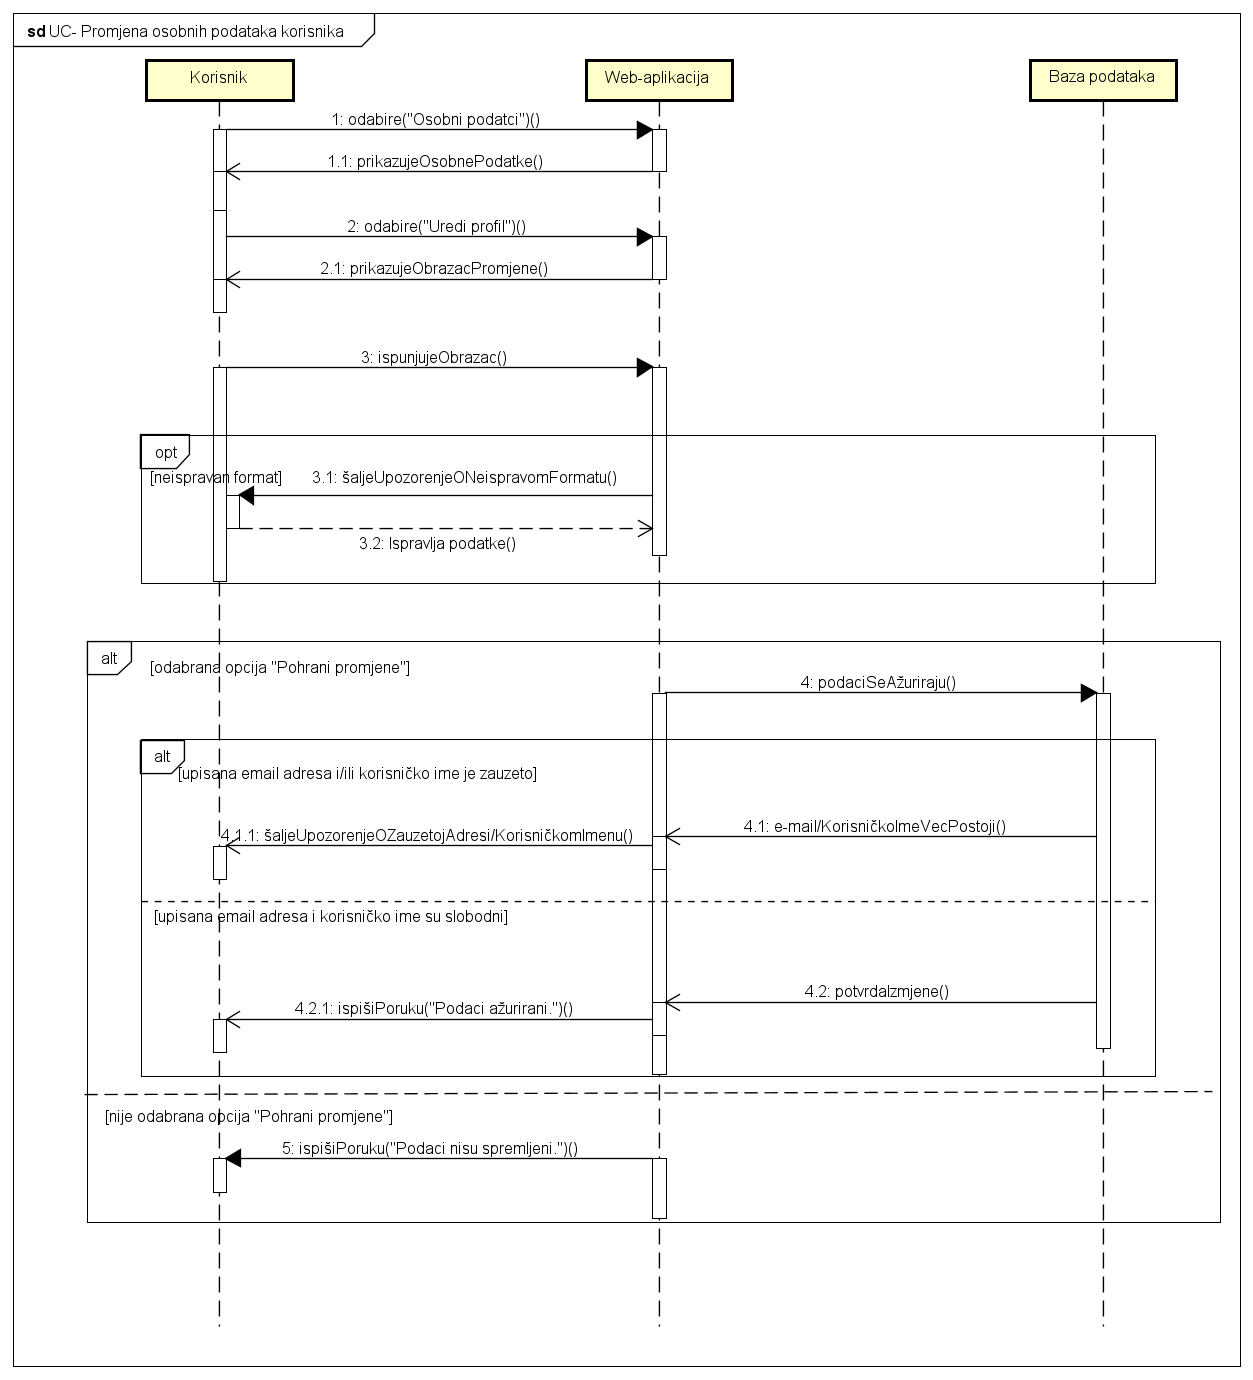
\includegraphics[scale=0.5]{dijagrami/UC8.png} %veličina u odnosu na širinu linije
				\caption{Sekvencijski dijagram: UC8 - Promjena osobnih podataka korisnika}
				\label{fig:UC8} %label mora biti drugaciji za svaku sliku
			\end{figure}
		
			\newpage
		
		
			\subsubsection{Obrazac uporabe UC10: Dodavanje novog profila psa u listu prijavljene udruge}
			
			Korisnik (koji je prijavljena udruga) na izbornoj traci odabire opciju "Moji psi". Aplikacija od baze dohvaća listu pasa te ju prikazuje korisniku. Korisnik odabire opcija "Dodaj novog psa" u tom prozoru te mu aplikacija vraća prazni obrazac. Korisnik ispuni obrazac te odabire opciju "Dodaj psa". U slučaju da je neki od podataka u neispravnom obliku, aplikacija upozorava korisnika da podaci nisu spremljeni jer su u neispravnom formatu. Korisnik tada ispravlja podatke i ponovno ih šalje. Jednom kada su podaci ispravni, baza vraća potvrdu o unosu podataka te aplikacija vraća korisniku poruku da je dodan novi pas. U slučaju da korisnik izlazi prije uspješnog dodavanja novog psa, aplikacija mu šalje upozorenje da novi pas nije dodan.
			
			\begin{figure}[H]
			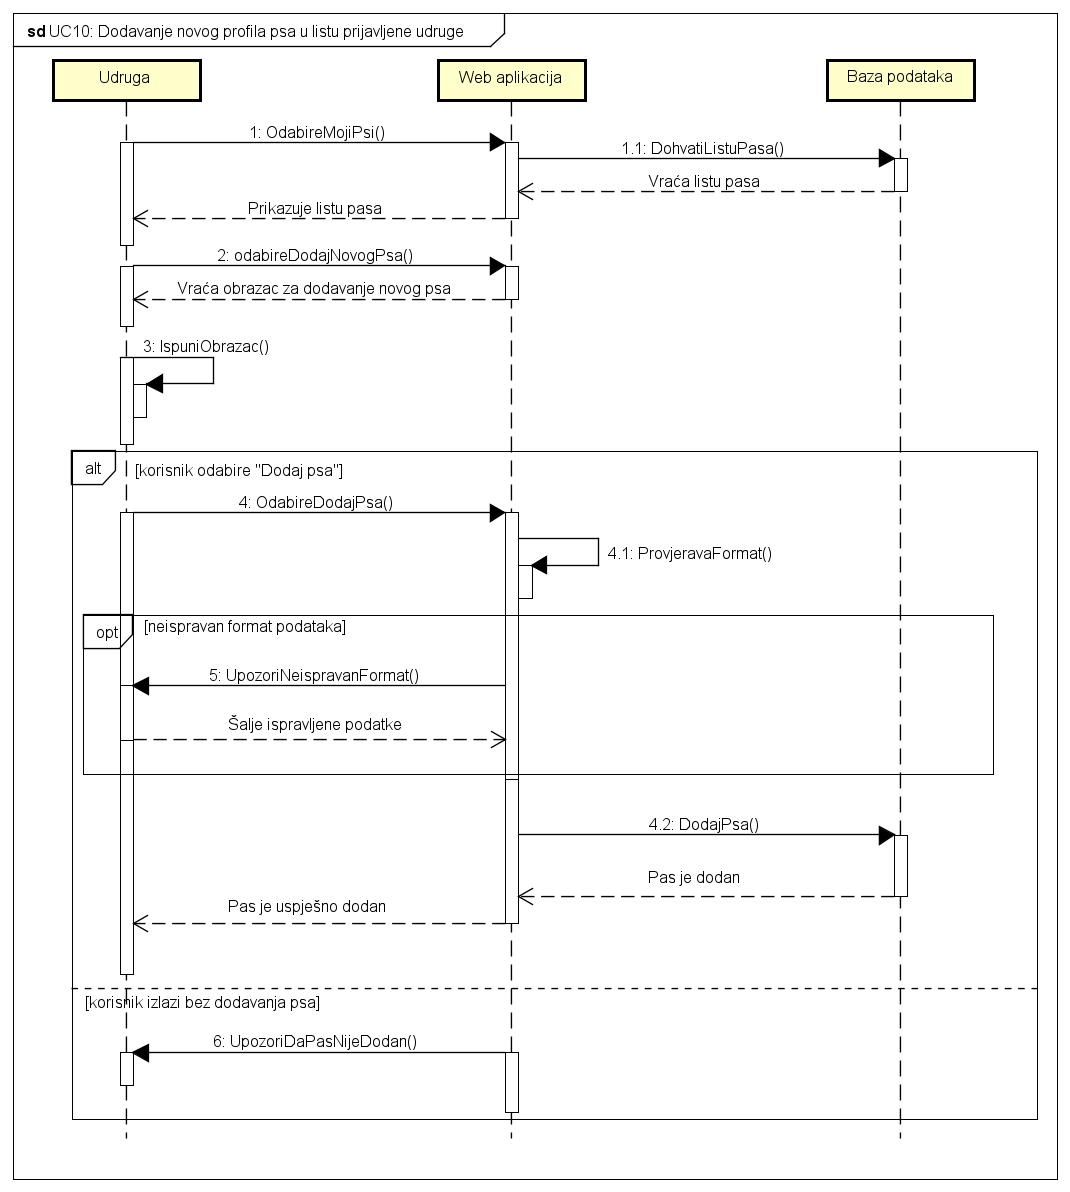
\includegraphics[scale=0.6]{dijagrami/UC10.png} %veličina u odnosu na širinu linije
			\caption{Sekvencijski dijagram: UC10 - Dodavanje novog profila psa u listu prijavljene udruge}
			\label{fig:UC10} %label mora biti drugaciji za svaku sliku
			\end{figure}
		
			\newpage
	
	
			\subsubsection{Obrazac uporabe UC13: Rezervacija termina šetnje}
			
			Korisnik (koji je građanin) može pregledati pse na dva načina:
			\begin{itemize}
				\item preko liste svih pasa:
				\begin{itemize}
					\item korisnik na izbornoj traci odabire "Psi"
					\item aplikacija od baze dohvaća sve pse
					\item korisniku je sada prikazana lista pasa iz svih udruga
				\end{itemize}
				\item preko liste pasa određene udruge:
				\begin{itemize}
					\item korisnik na izbornoj traci odabire "Udruge"
					\item aplikacija od baze dohvaća sve udruge te prikazuje korisniku listu svih udruga
					\ korisnik odabire udrugu
					\item aplikacija od baze dohvaća listu svih pasa iz odabrane udruge te ih prikazuje korisniku
				\end{itemize}
			\end{itemize}
			Nakon otvaranja liste pasa, korisnik bira psa kojeg bi volio šetati. Aplikacija od baze dohvaća profil (informacije) te raspored željenog psa te ih prikazuje korisniku. Korisnik bira željeni termin šetnje te aplikacija šalje rezervaciju bazi. Baza potvrđuje unos te aplikacija korisniku potvrđuje rezervaciju.
			
			
			\begin{figure}[H]
				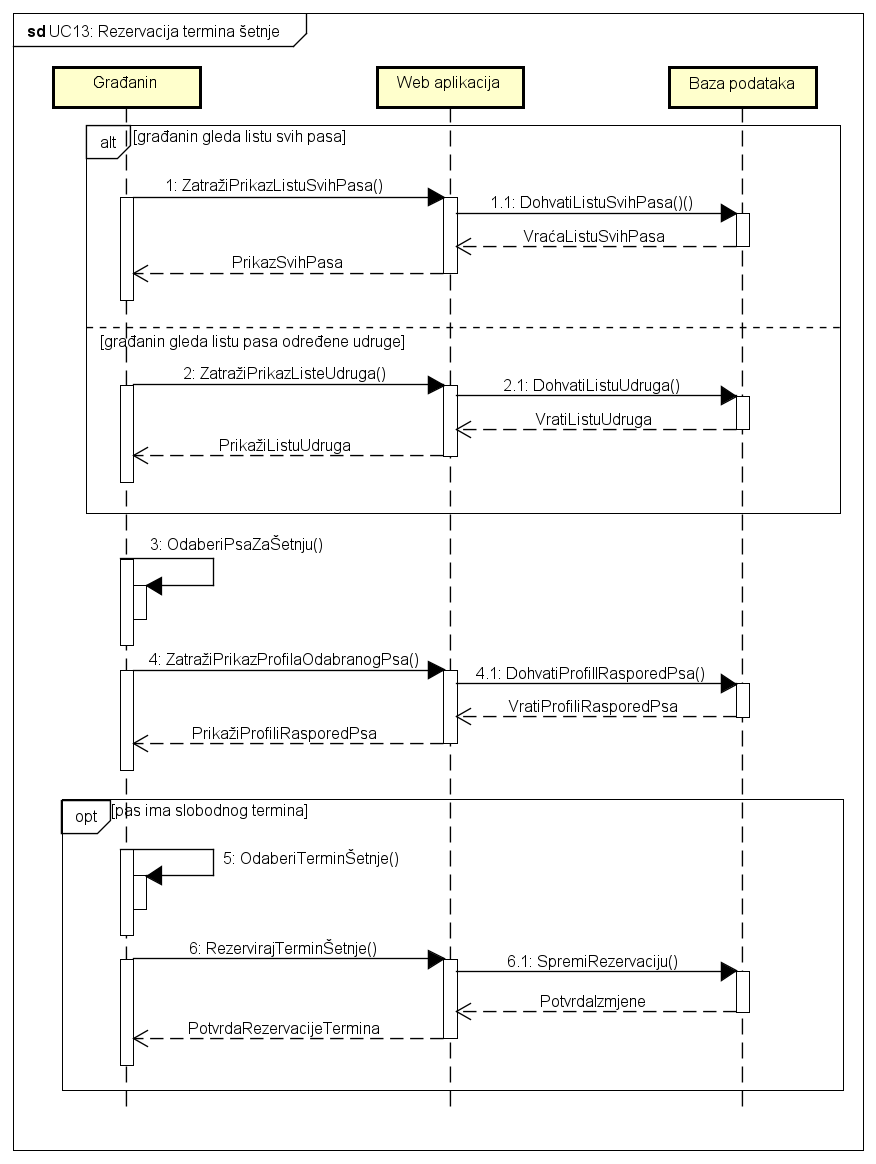
\includegraphics[scale=0.68]{dijagrami/UC13.png} %veličina u odnosu na širinu linije
				\caption{Sekvencijski dijagram: UC13 - Rezervacija termina šetnje}
			\label{fig:UC13} %label mora biti drugaciji za svaku sliku
			\end{figure}
	
			\subsubsection{Obrazac uporabe UC15: Označavanje statistike šetnji kao javne}
			
			Korisnik (koji je građanin) odabire opciju "Moj profil" sa izborne trake. Web aplikacija dohvaća od baze podatke o korisniku te ih vraća. Aplikacija prikazuje korisniku njegove podatke. Korisnik odabire opciju "Moja statistika". Aplikacija od baze dohvaća podatke o obavljenim štenjama korisnika te ih prikazuje. U tom prozoru postoji opcija "Označi svoju statistiku javnom" te korisnik odabire tu opciju. Statistika postaje vidljiva u rang-listi svih šetača.
	
			\begin{figure}[H]
			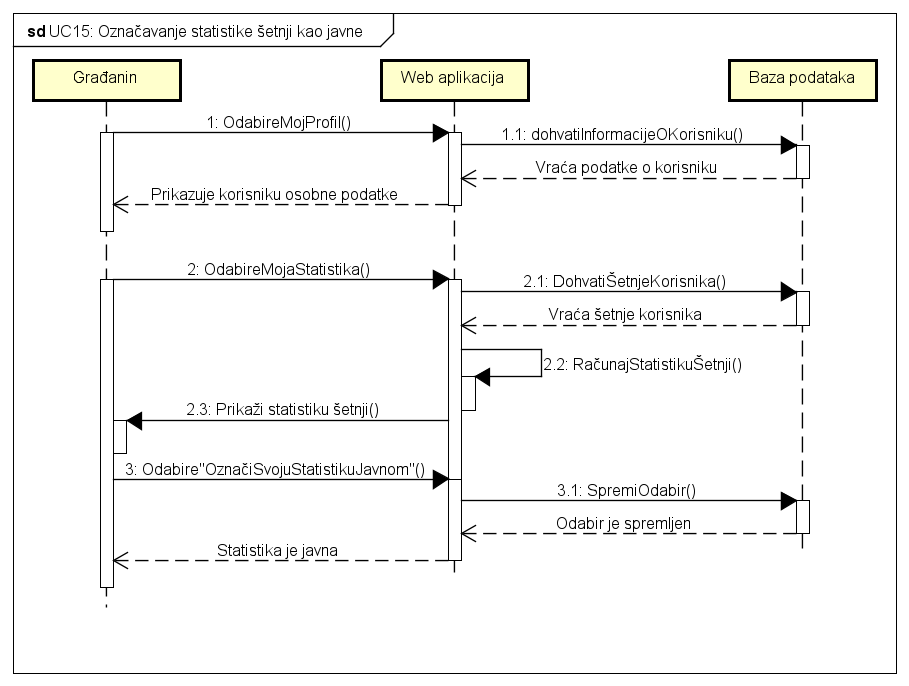
\includegraphics[scale=0.67]{dijagrami/UC15.png} %veličina u odnosu na širinu linije
			\caption{Sekvencijski dijagram: UC15 - Označavanje statistike šetnji kao javne}
			\label{fig:UC15} %label mora biti drugaciji za svaku sliku
			\end{figure}
	
		\newpage
		
	\section{Ostali zahtjevi}
	
	\iffalse
	
		\textbf{\textit{dio 1. revizije}}\\
 
	 \textit{Nefunkcionalni zahtjevi i zahtjevi domene primjene dopunjuju funkcionalne zahtjeve. Oni opisuju \textbf{kako se sustav treba ponašati} i koja \textbf{ograničenja} treba poštivati (performanse, korisničko iskustvo, pouzdanost, standardi kvalitete, sigurnost...). Primjeri takvih zahtjeva u Vašem projektu mogu biti: podržani jezici korisničkog sučelja, vrijeme odziva, najveći mogući podržani broj korisnika, podržane web/mobilne platforme, razina zaštite (protokoli komunikacije, kriptiranje...)... Svaki takav zahtjev potrebno je navesti u jednoj ili dvije rečenice.}
	 
	 \fi
	 
	 \begin{packed_item}
	 	\item Sustav treba omogućiti rad više korisnika u stvarnom vremenu 
	 	\item  Korisničko sučelje i sustav moraju podržavati hrvatsku abecedu (dijakritičke znakove) pri unosu i prikazu tekstualnog sadržaja
	 	\item  Izvršavanje dijela programa u kojem se pristupa bazi podataka ne smije trajati duže od nekoliko sekundi
	 	\item  Sustav treba biti implementiran kao web aplikacija koristeći objektno-orijentirane jezike
	 	\item  Neispravno korištenje korisničkog sučelja ne smije narušiti funkcionalnost i rad sustava
	 	\item  Sustav treba biti jednostavan za korištenje, korisnici se moraju znati koristiti sučeljem bez opširnih uputa
	 	\item  Nadogradnja sustava ne smije narušavati postojeće funkcionalnosti sustava
	 	\item  Veza s bazom podataka mora biti kvalitetno zastićena, brza i otporna na vanjske greške
	 	\item  Pristup sustavu mora biti omogućen iz javne mreže pomoću HTTPS. 
	 	\item S obzirom da je aplikacija na hrvatskom, datum prikazuje na odgovarajući način: DD.MM.YYYY.
	 \end{packed_item}
	 
